% Packages

\documentclass[
	11pt, % Set the default font size, options include: 8pt, 9pt, 10pt, 11pt, 12pt, 14pt, 17pt, 20pt
	%t, % Uncomment to vertically align all slide content to the top of the slide, rather than the default centered
	%aspectratio=169, % Uncomment to set the aspect ratio to a 16:9 ratio which matches the aspect ratio of 1080p and 4K screens and projectors
]{beamer}
\setcounter{tocdepth}{1}
\usepackage{graphicx}
\usepackage[export]{adjustbox}
\graphicspath{{Images/}{./}} % Specifies where to look for included images (trailing slash required)
\usepackage{tikz}
\newenvironment{amatrix}[1]{%
  \left[\begin{array}{@{}*{#1}{c}|c@{}}
}{%
  \end{array}\right]
}

\usepackage{booktabs} % Allows the use of \toprule, \midrule and \bottomrule for better rules in tables
\usepackage{pgfplots}
\usepackage{tikz}
\pgfplotsset{width=6cm, compat=newest, every tick label/.append style={scale=0.5}}
\usepackage{amsmath}
\usepackage{blkarray}% http://ctan.org/pkg/blkarray
\newcommand{\matindex}[1]{\mbox{\scriptsize#1}}% Matrix index

% Theme
\usetheme{Madrid}

% Font
\usefonttheme{serif}
\usepackage{newtxtext,newtxmath}
\usepackage[default]{lato}

% Inner theme
\useinnertheme{circles}

% Information
\title{Logic}
\author{Kin Hei Wong}
\date{\today}
%%%%%%%%%%%%%%%%%%%%%%%%%%%%%%%%%%%%%%%%%%%%%%%%%%%%%%%%%%
\begin{document}
% Title slide
\begin{frame}
    \titlepage
\end{frame}

% Table of Content
\begin{frame}
    \frametitle{Presentation overview}
    \tableofcontents
\end{frame}
%%%%%%%%%%%%%%%%%%%%%%%%%%%%%%%%%%%%%%%%%%%%%%%%%%%%%%%%%%%
% Body slides
\section{7A: The algebra of sets}
\begin{frame}
    \frametitle{7A}
    \begin{center}
        \title{The algebra of sets}
        \maketitle
    \end{center}
\end{frame}

\begin{frame}[t]
    \frametitle{All subset of a set}
    It always apply $2^n$ when a set has $n$ element.\\
    E.g. $\xi = {a, b, c, d}$
\end{frame}


\begin{frame}
    \frametitle{Axioms}
    \begin{center}
        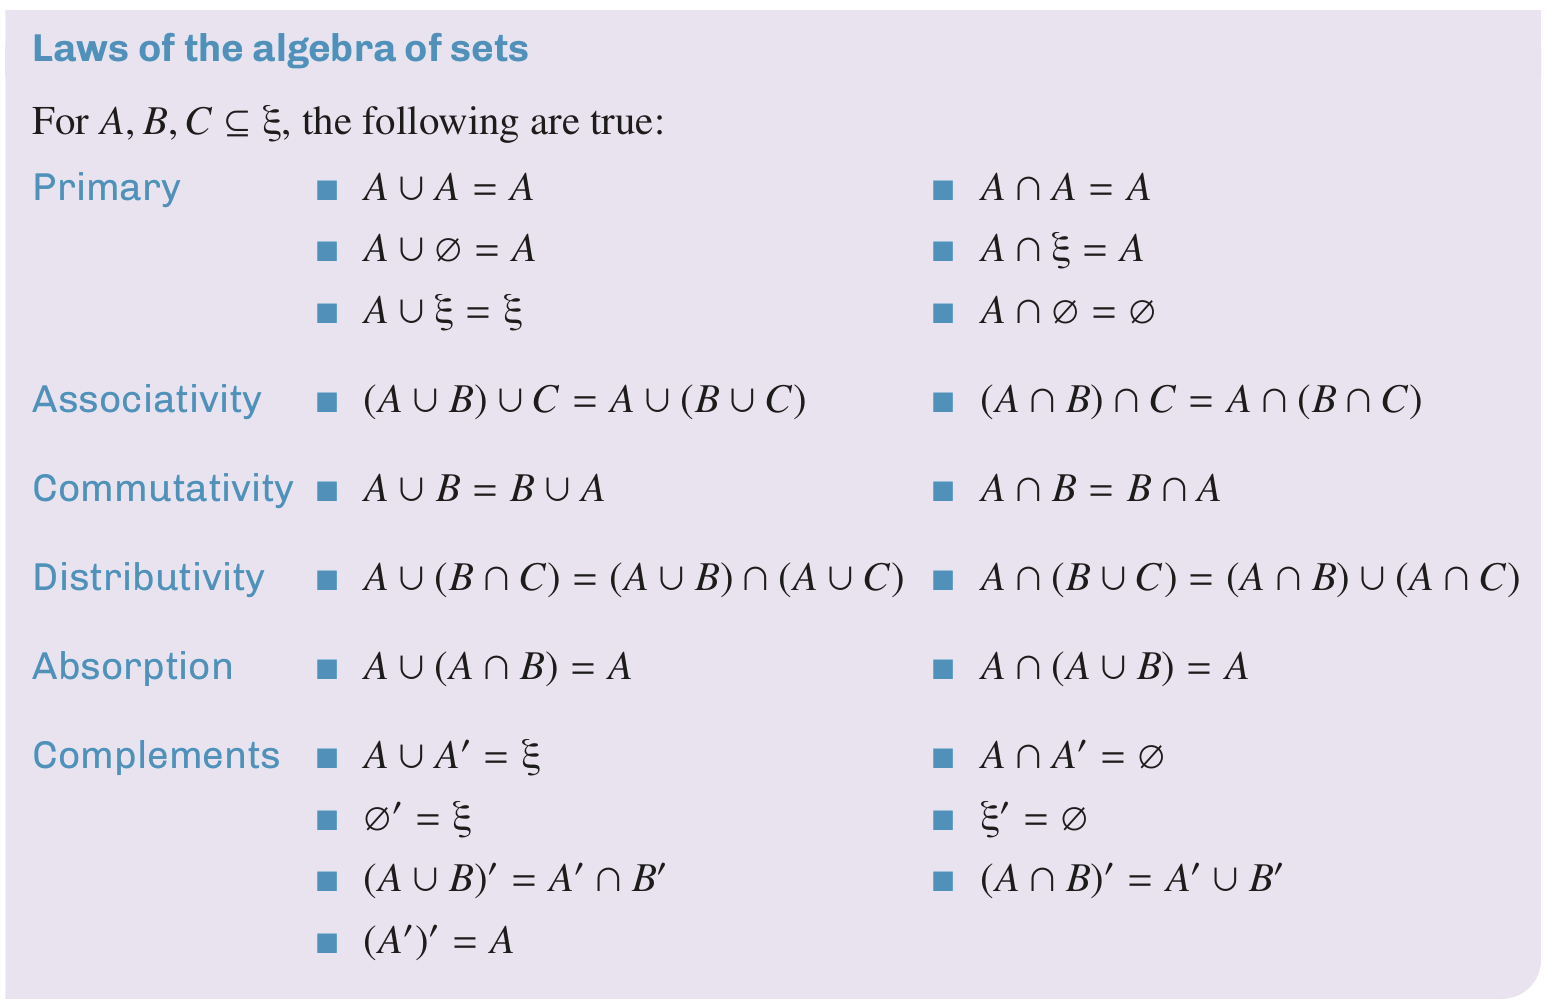
\includegraphics[width = 8cm]{Axioms.png}\\
        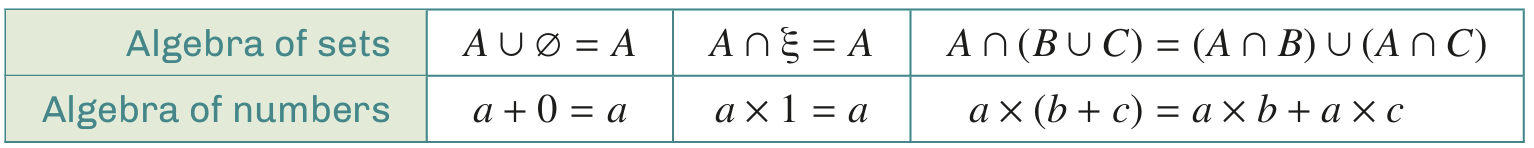
\includegraphics[width = 8cm]{Sim.png}
    \end{center}
\end{frame}

\begin{frame}[t]
    \frametitle{Example 1}
    \begin{center}
        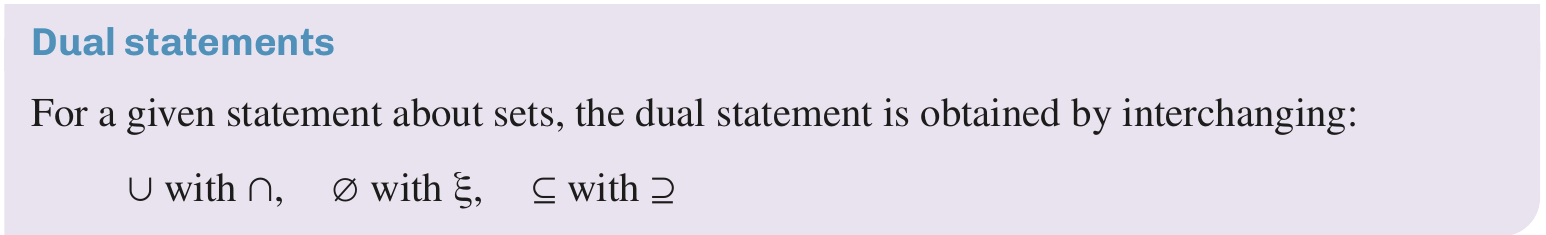
\includegraphics[width = 8cm]{Dual.png}
    \end{center}
    Write the dual of $(A \cap B')\cap B = \emptyset$.  
\end{frame}

\begin{frame}[t]
    \frametitle{Example 2}
    \begin{block}{Equality for sets}
        When proving that two sets are equal, we can use the following equivalence:\\
        $X\subseteq Y \text{ and } Y \subseteq X \iff X = Y$
    \end{block}
    \begin{enumerate}
        \item Illustrate $(A\cup B)' = A' \cap B'$ with Venn diagram.
        \item Prove $(A\cup B)' = A' \cap B'$.
    \end{enumerate}
\end{frame}
\begin{frame}
\end{frame}

\begin{frame}[t]
    \frametitle{Example 3}
    Simplify each of the following expressions:\\
    \begin{enumerate}
        \item $X \cap (Y \cap X')$
        \item $X' \cup (Y \cap X)$
        \item $[X' \cup (Y \cap X)']$
        \item $[(X \cap Y') \cup (X \cap Y)]'$
    \end{enumerate}
\end{frame}

\begin{frame}
\end{frame}

\begin{frame}
    \frametitle{Exercise 7A}
\end{frame}

%%%%%%%%%%%%%%%%%%%%%%%%%%%%%%%%%%%%%%%%%%%%%%%%%%%%%%%%%%%
% Body slides
\section{7B: Switching circuits}
\begin{frame}
    \frametitle{7B}
    \begin{center}
        \title{Switching circuits}
        \maketitle
    \end{center}
\end{frame}

\begin{frame}
    \frametitle{Circuits table}
    \begin{center}
        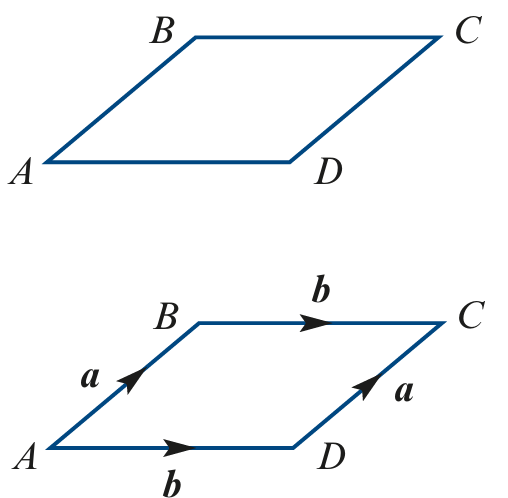
\includegraphics[width = 8cm]{Parallel.png}\\
        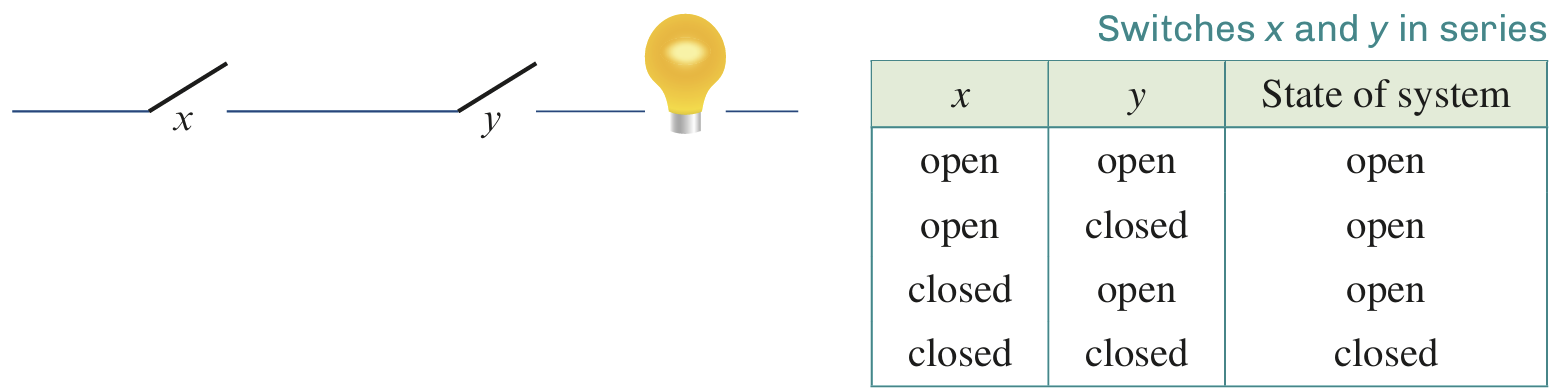
\includegraphics[width = 8cm]{Series.png}
    \end{center}
\end{frame}

\begin{frame}[t]
    \frametitle{New notation}
    Open circuit: 0\\
    Closed circuit: 1\\
    $x \cup y = x \lor y$\\
    $x \cap y = x \land y$\\
    $x'$ for complement
\end{frame}

\begin{frame}[t]
    \frametitle{Example 4}
    Evaluate ($1 \lor 0) \land 1'$.
\end{frame}

\begin{frame}[t]
    \frametitle{Example 5}
    Consider the expression\\
    $(x \land y) \lor (z \land x')$\\
    \begin{enumerate}
        \item Draw the switching circuit that is represented by this expression
        \item Give a table that describes the operation of this circuit for all possible combinations of switches $x, y$ and $z$ being open (0) and closed (1).
    \end{enumerate}
\end{frame}

\begin{frame}
    \frametitle{Exercise 7B}
\end{frame}

%%%%%%%%%%%%%%%%%%%%%%%%%%%%%%%%%%%%%%%%%%%%%%%%%%%%%%%%%%%
% Body slides
\section{7C: Boolean algebra}
\begin{frame}
    \frametitle{7C}
    \begin{center}
        \title{Boolean algebra}
        \maketitle
    \end{center}
\end{frame}

\begin{frame}
    \frametitle{More axioms}
    \begin{enumerate}
        \item A1(Commutative): $x \lor y = y \lor x$\quad|\quad$x \land y = y \land x$
        \item A2(Associative): $(x \lor y) \lor z = x \lor (y \lor z)$\quad|\quad$(x \land y) \land z = x \land (y \land z)$
        \item A3: $x \lor (y \land z) = (x \lor y) \land (x \lor z)$\quad|\quad$x \land (y \lor z) = (x \land y) \lor (x \land z)$
        \item A4: $x\lor 0 = x$\quad|\quad $x\land 1 = x$
        \item A5(Complementation): $x \lor x' = 1$\quad|\quad $x \lor x' = 0$
    \end{enumerate}
\end{frame}

\begin{frame}[t]
    \frametitle{Example 6}
    Prove that, for each Boolean algebra B and all $x,y,a,b\in B$:\\
    \begin{enumerate}
        \item $x \lor 1 = 1$
        \item $x \land 0 =0$
        \item If $a \lor b = 1$ and $a \land b = 0$, then $a'=b'$.
        \item $(x \lor y)' = x' \land y'$
    \end{enumerate}
\end{frame}
\begin{frame}
\end{frame}
\begin{frame}
    \frametitle{Properties of Boolean algebras}
    \begin{center}
        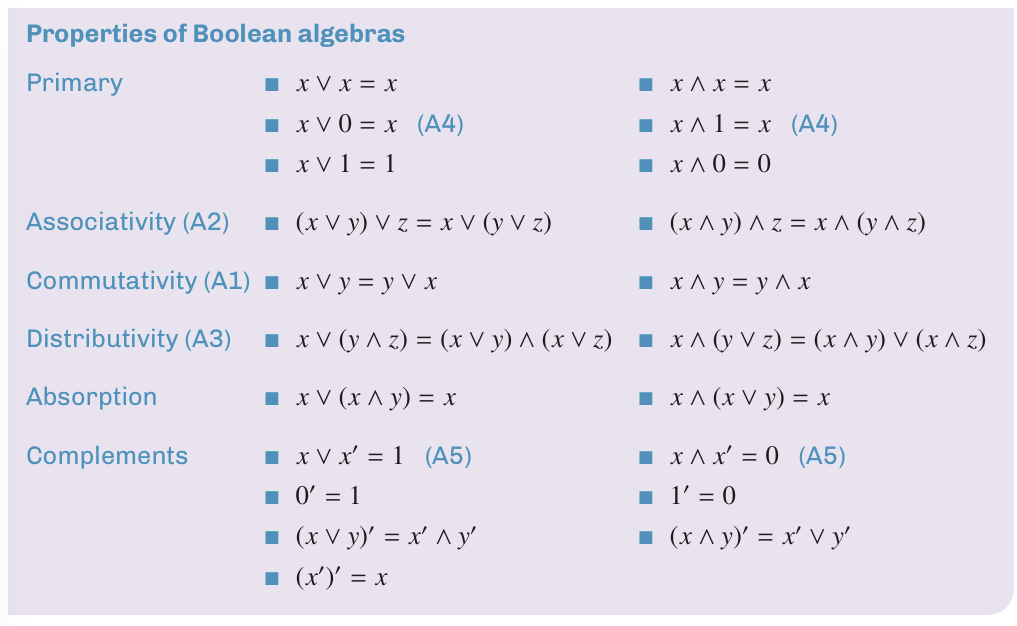
\includegraphics[width = 8cm]{Boolean.png}
    \end{center}
\end{frame}

\begin{frame}[t]
    \frametitle{Example 7}
    \begin{block}{Boolean expressions and functions}
        $f:{0,1} \rightarrow {0, 1}$, \qquad $f(x) = x \lor 1$\\
        In this case, we have $f(0) = 0 \lor 1 = 1$ and $f(1) = 1\lor 1 = 1$.
        In general, a Boolean function has one or more inputs from ${0, 1}$ and outputs in ${0, 1}$.
    \end{block}
    Give the table of values for the Boolean function $f(x,y) = (x\land y)\lor y'$.
\end{frame}

\begin{frame}[t]
    \frametitle{Example 8}
    Find a Boolean expression for the Boolean function given by the following table.\\
    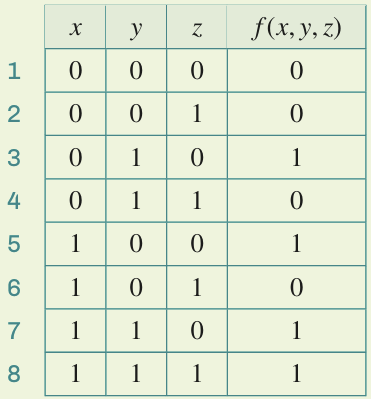
\includegraphics[width = 4cm]{Ex8.png}
\end{frame}
\begin{frame}
\end{frame}

\begin{frame}[t]
    \frametitle{Example 9}
    \begin{block}{Equivalent Boolean expressions}
        Two Boolean expressions are \textbf{equivalent} if they represent the same Boolean function.        
    \end{block}
    Consider the two Boolean expressions\\
    $((x \lor y) \land (x' \lor y)) \lor x$ and $x \lor y$\\
    Show that these two expressions are equivalent by:\\
    \begin{enumerate}
        \item showing that they represent the same Boolean function
        \item using the axioms and properties of Boolean algebras
    \end{enumerate}
\end{frame}

\begin{frame}
    \frametitle{Exercise 7C}
\end{frame}

%%%%%%%%%%%%%%%%%%%%%%%%%%%%%%%%%%%%%%%%%%%%%%%%%%%%%%%%%%%
% Body slides
\section{7D: Logical connectives and truth tables}
\begin{frame}
    \frametitle{7D}
    \begin{center}
        \title{Logical connectives and truth tables}
        \maketitle
    \end{center}
\end{frame}

\begin{frame}
    \frametitle{What is a statement?}
    A statement is a sentence that is either true or false. Examples of statments are:\\
    \begin{enumerate}
        \item The boy plays tennis
        \item 5 + 7 = 12
        \item 5 + 7 = 10
    \end{enumerate}
\end{frame}

\begin{frame}[t]
    \frametitle{Logical: 'or', 'and', 'not'}
    Let G be the statement '$n$ is odd', H be the statement '$n>10$'
    \begin{columns}
        \begin{column}{0.333\textwidth}
            \textbf{Or (Disjoint)}
        \end{column}
        \begin{column}{0.333\textwidth}
            \textbf{And (Conjoint)}
        \end{column}
        \begin{column}{0.333\textwidth}
            \textbf{Not (Negation)}
        \end{column}
    \end{columns}
\end{frame}

\begin{frame}[t]
    \frametitle{Example 10}
    Write the truth table for $\lnot(A \lor B)$.
\end{frame}

\begin{frame}[t]
    \frametitle{Example 11}
    Write the truth table for $(A\land B) \land (\lnot A)$.
\end{frame}

\begin{frame}[t]
    \frametitle{Example 12}
    Show that $\lnot(A \land B)$ is logically equivalent to $\lnot A \lor \lnot B$.
\end{frame}

\begin{frame}[t]
    \frametitle{Example 13}
    Show that $(\lnot A) \lor (A \lor B)$ is a tautology.
\end{frame}

\begin{frame}[t]
    \frametitle{Example 14}
    Show that $(A \lor B) \land (\lnot A \land \lnot B)$ is a contradiction.
\end{frame}

\begin{frame}[t]
    \frametitle{Implication}
    Implication is probably one of the most confusing logical connective.\\
    It understands as If A, then B, notation as: $A \implies B$. \\
    E.g.\\
    A = 'I am elected'\\
    B = 'I will make public tranport free'
\end{frame}

\begin{frame}[t]
    \frametitle{Example 15}
    Give the truth table for $B \implies (A \lor \lnot B)$.
\end{frame}

\begin{frame}[t]
    \frametitle{Example 16}
    Give the truth table for $(\lnot A \lor \lnot B) \iff \lnot (A \land B).$.
\end{frame}

\begin{frame}[t]
    \frametitle{Negation of implication}   
    Try writing down a negation of the conditional statement $A\implies B$. What do you realise?
\end{frame}

\begin{frame}[t]
    \frametitle{Example 17}
    For each of the following conditional statements:
    \begin{enumerate}
        \item write the converse
        \item write the contrapositive
        \item write the negation
        \begin{enumerate}
            \item If you know the password, then you can get in.
            \item Let $n,a,b \in \mathbb{N}$. If $n$ does not divide $ab$, then $n$ does not divide $a$ and $n$ does not divide b.
        \end{enumerate}
    \end{enumerate}
\end{frame}

\begin{frame}
    \frametitle{The Boolean algebra of statements}
    We use equivalence ($\equiv$) instead of equality (=). E.g.\\
    $A \lor \lnot A \equiv T$\quad and \quad $A \land \lnot A \equiv F$ 
\end{frame}

\begin{frame}
    \frametitle{Exercise 7D}
\end{frame}

%%%%%%%%%%%%%%%%%%%%%%%%%%%%%%%%%%%%%%%%%%%%%%%%%%%%%%%%%%%
% Body slides
\section{7E: Valid argument}
\begin{frame}
    \frametitle{7E}
    \begin{center}
        \title{Valid argument}
        \maketitle
    \end{center}
\end{frame}

\begin{frame}[t]
    \frametitle{Example 18}
    By constructing a truth table, decide whether or not the following argument is valid.\\
    Premise 1: If Australia is democracy, then Australians have the right to vote.\\
    Premise 2: Australia is a democracy.\\
    Conclusion: Australians have the right to vote.
\end{frame}

\begin{frame}[t]
    \frametitle{Example 19}
    By constructing a truth table, decide whether or not the following argument is valid.\\
    Premise 1: If you invest in Company W, then you get rich.\\
    Premise 2: You did not invest in Company W.\\
    Conclusion: You did not get rich.
\end{frame}

\begin{frame}
    \frametitle{Valid arguments with false conclusions}
    Premise 1: If 2 is odd, then 3 is even.\\
    Premise 2: The number 2 is odd.\\
    Conclusion: The number 3 is even
\end{frame}

\begin{frame}
    \frametitle{Invalid argument with true conclusions}
    Premise 1: If 2 is odd, then 3 is even.\\
    Premise 2: The number 2 is even.\\
    Conclusion: THe number 3 is odd.
\end{frame}

\begin{frame}[t]
    \frametitle{Checking for tautology - Example 20}
    Investigate the validity of each of the following arguments by checking whether or not an
    appropriate compound statement is a tautology:\\
    \begin{enumerate}
        \item In March, there are strong winds every day. The wind is not strong today. Therefore it
        is not March.
        \item  On Mondays I go swimming. Today is not Monday. Therefore I do not swim today.
    \end{enumerate}
\end{frame}
\begin{frame}
\end{frame}

\begin{frame}
    \frametitle{Exercise 7E}
\end{frame}

%%%%%%%%%%%%%%%%%%%%%%%%%%%%%%%%%%%%%%%%%%%%%%%%%%%%%%%%%%%
% Body slides
\section{7F: Logic circuits}
\begin{frame}
    \frametitle{7F}
    \begin{center}
        \title{Logic circuits}
        \maketitle
    \end{center}
\end{frame}

\begin{frame}
    \frametitle{Logic gates}
    If you are about to study/studying electricity, you are in luck. This is basic for you.\\
    \begin{center}
        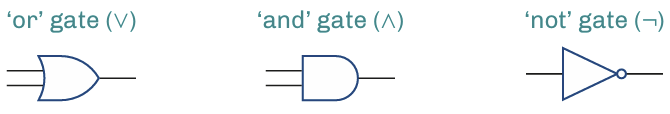
\includegraphics[width = 8cm]{Gates.png}
    \end{center}
\end{frame}

\begin{frame}[t]
    \frametitle{Example 21}
    Give the gate representation of the Boolean expression $(A \land B) \lor C$.
\end{frame}

\begin{frame}[t]
    \frametitle{Example 22}
    \begin{enumerate}
        \item Give the gate representation of the Boolean expression $A \lor (\lnot A \land B)$.
        \item Describe the operation of this circuit through a truth table.
    \end{enumerate}
\end{frame}

\begin{frame}[t]
    \frametitle{Example 23}
    Consider the truth table shown below.\\
    \begin{enumerate}
        \item Using the technique from Example 8, construct a Boolean expression to match this truth table.
        \item Draw a circuit for this expressions.
        \item Use the properties of Boolean algebras to simplify the expression, and hence draw a simpler circuit that is equivalent to the circuit from b.
    \end{enumerate}
    \begin{center}
        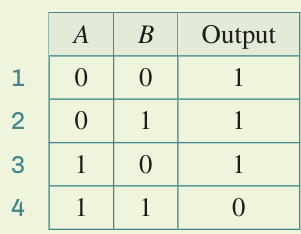
\includegraphics[width = 4cm]{Ex23.png}
    \end{center}
\end{frame}
\begin{frame}
\end{frame}

\begin{frame}
    \frametitle{Exercise 7F}
\end{frame}

%%%%%%%%%%%%%%%%%%%%%%%%%%%%%%%%%%%%%%%%%%%%%%%%%%%%%%%%%%%
% Body slides
\section{7G: Karnaugh maps}
\begin{frame}
    \frametitle{7G}
    \begin{center}
        \title{Karnaugh maps}
        \maketitle
    \end{center}
\end{frame}

\begin{frame}
    \frametitle{Minimal representation}
    Karnaugh maps allow to have more simpler circuit by more compact and cheaper to produce from Boolean expressions.\\
    \begin{block}{Minimal representation}
        Let $f$ be a non-constant Boolean function. Then a \textbf{minimal representation} of $f$ is a Boolean expression $E$ which represents $f$ and satisfies the following:\\
        \begin{enumerate}
            \item The expression $E$ has the form $E_1 \lor E_2 \lor \dots E_n$, where each $E_i$ is an expression such as $x \land y$ or $x' \land y' \land z$ or $y \land z'$.
            \item If $F$ is any other expression of this form which also represents $f$, then the number of terms $F_i$ is greater than or equal to the number of terms $E_i$.
            \item If $F$ and $E$ have the same number of terms, then the number of variables in F is greater than or equal to the number of variables in $E$.
        \end{enumerate}
    \end{block}
\end{frame}

\begin{frame}[t]
    \frametitle{Two variables}
    Try writing the truth table for $f(x,y) = (x' \land y') \lor (x' \land y) \lor (x \land y)$.
\end{frame}

\begin{frame}[t]
    \frametitle{Karnaugh map calculation}
    $(x' \land y') \lor (x' \land y) \lor (x \land y)$=
\end{frame}

\begin{frame}[t]
    \frametitle{Example 24}
    Simplify $(x \land y) \lor (x \land y') \lor (x' \land y)$.
\end{frame}

\begin{frame}
    \frametitle{Rules for using Karnaugh maps}
    \begin{block}{Blocks in Karnaugh maps}
        \begin{enumerate}
            \item You may use an $m \times n$ block in a Karnaugh map if both $m$ and $n$ are powers of 2. (So you may use $1 \times 1, 1 \times 2, 1 \times 4, 2 \times 1, 2 \times 2, 2 \times 4)$
            \item You always try to form the biggest blocks that you can, and to use the least number of blocks that you can.
        \end{enumerate}
    \end{block}
    \begin{center}
        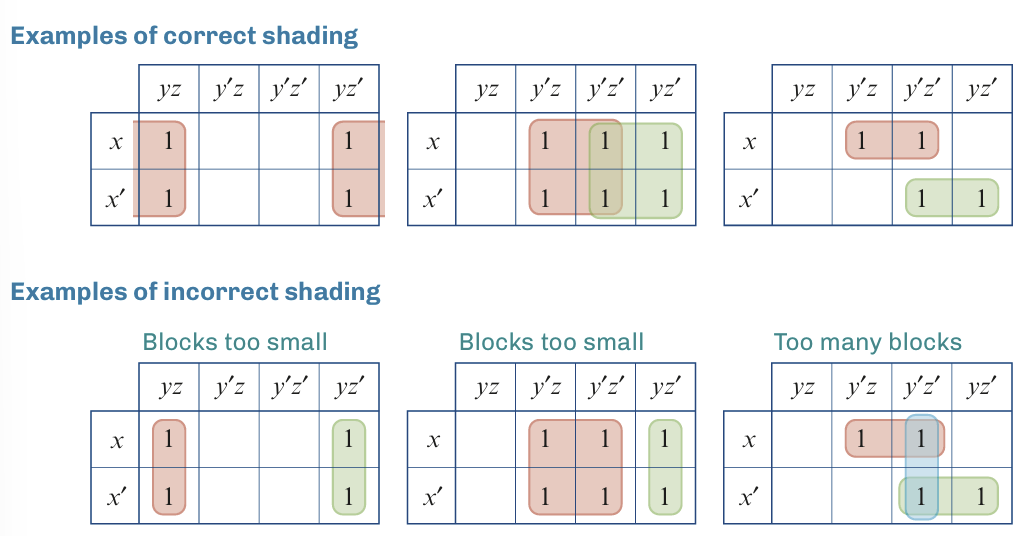
\includegraphics[width = 8cm]{Shading.png}
    \end{center}
\end{frame}

\begin{frame}[t]
    \frametitle{Example 25}
    Simplify $(x \land y \land z) \lor (x\land y \land z') \lor (x\land y' \land z')\lor (x' \land y \land z')$.
\end{frame}

\begin{frame}[t]
    \frametitle{Example 26}
    Write a minimal Boolean expression for the following truth table.\\
    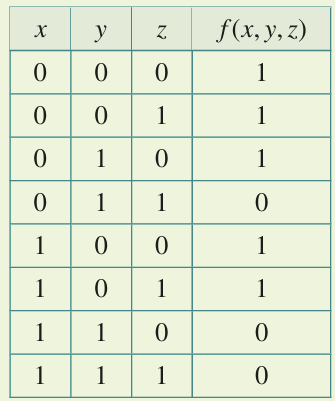
\includegraphics[width = 4cm]{Ex26.png}
\end{frame}

\begin{frame}
    \frametitle{Exercise 7G}
\end{frame}

\end{document}